\chapter{Conclusion}

This chapter briefly summarises the approach of this thesis, and then goes on to sum up the key findings from the field works. Finally, the thesis concludes with limitations and an outlook on future work that this thesis might inspire.\\

\section{Summary of approach}
This PhD work use Mixed reality game - AtomicOrchid as a testbed to probe the design implications for agent planning support system. Field trials were conducted for the three versions of AtomicOrchid game with different interaction design patterns. The first one is a non agent version of the game. The second and third studies are planned to probe two interaction design patterns (On-the-loop and In-the-loop). Video and system logs of the field trails has been collected and interaction analysis has been conducted to generate requirements and interaction design implications. \\


\section{Summary of findings}
Three studies are carried out iteratively. The AtomicOrchid system evolves throughout the three studies. The interaction design for the study 2 and 3 follows the design patterns (On-the-loop and In-the-loop), but are also inspired by key observations from previous studies. The key observations leads to both interactional issues and detailed system requirements which inspires system evolution across the three trials (see figure \ref{fig:connections}).  The section \ref{sec:conclusionIE}  will give details about how the system evolves and the interface design rationales. The interactional issues emerged from field observations will be detailed in section\ref{sec:conclusionIssue}.  In what follows, the section will give a brief overview of the key observations from the three studies.\\ 


\begin{figure}[h]
  \centering
  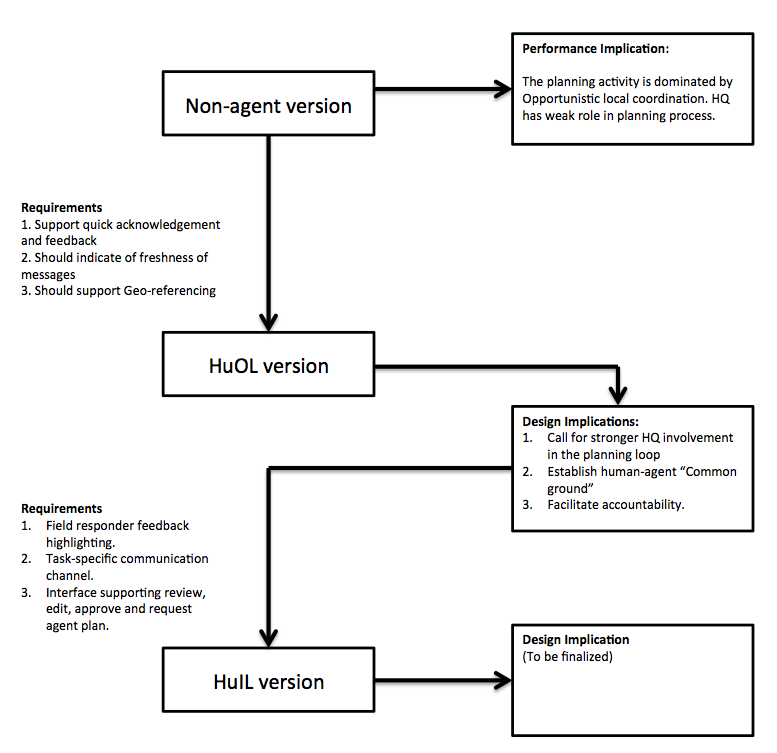
\includegraphics[width=1\textwidth]{img/conclusion/connections}
  \caption{ Interaction issues and interface improvements}
  \label{fig:connections}
\end{figure}

The non-agent AtomicOrchid trial (study 1) is aimed to give insight into how human conduct planning (without agent support) in the time and spatially constrained disaster settings and to generate general requirements of coordination support system which is also applicable to the next two agent-integrated version of AtomicOrchid. The result of interaction analysis showed the team planning is dominated by local coordination between field players with in an ``ad-hoc'' manner. The field teams managed organise their team and task allocations without conflicts. The HQ is found to successfully provide awareness of the ``danger zone'' to the field teams. However, they have little influence on the planning activities of the team. One potential reason could be the breakdown of communication between HQ and Field responders. The communication is thought to be affected by a set of factors including communication modalities (text vs voice), training level of players and HQ and system interface designs. A number of system requirements has also be introduced in the study 1 , which inspires system evolutions in the subsequent studies. \\


In study 2, a planning agent is integrated to the system with the HuOL interaction design. The general requirements from study 1 leads to a number of system improvements (see figure \ref{sec:conclusionIE}) in study 2, which help us to avoid non-agent related factors in field trials. Through interaction analysis, we gain insight into the division of labour between human and agent (see section \ref{sec:studytwointroduction}) in which the agent takes over routine planning activities while the human focus on other issues such as navigation. However, there are also evidence showing the agent planning occasionally interrupts workflow of human team because it fails to consider social cost of task changes. We also observed HQ player struggled to influence the plan because the lack of interface level support. Further, a set of misconceptions in feedback loops (see section \ref{sec:studytwofeedback}) are also observed.\\

In study 3, the system is evolved to facilitate In-the-loop interaction with the feedback from study 2. The main changes are a number of interface functionalities which enable HQ to approve, edit agent planning and monitor player feedbacks. Through observing the usage of this new functionalities in the control room, we found a new pattern division of labour between in which:
	\begin{enumerate}
	 \item The HQ decide when to perform re-plan.
	 \item The HQ review every agent instruction for routine task planning.
	 \item The planning agent deals with player feedback.
	 \item The Agent propose task allocation
	\end{enumerate}
	
Further observation shows that task interruptions caused by the agent planning (observed in study 2) may have been reduced as a result of greater HQ involvement in the planning. Analysis of some failed cases of coordination also points out a number of issues, which highlights potential human performance issues as a result of the greater HQ involvement in the planning. [ TO be finalised ]  \\

\section{Summary of interface evolutions}\label{sec:conclusionIE}
The section presents the interface evolutions of AtomicOrchid interface across three field studies and the design rationales behind it. The initial interface of AtomicOrchid (used in 1st study) is designed to display game status and provide broadcasting channel to support communication. In the first study, the control room is manned by 2-3 HQ players. Every HQ shares a same interface which shows game status on a map. A chat box is provided to send and receive broadcasting messages. The mobile interface is used by field responders. The responders share a same map with HQ, which displays game status with the exception of radioactive cloud. The messaging interface is placed in another tab.(see figure \ref{fig:study1interface})\\ 



\begin{figure}[H]
  \centering
  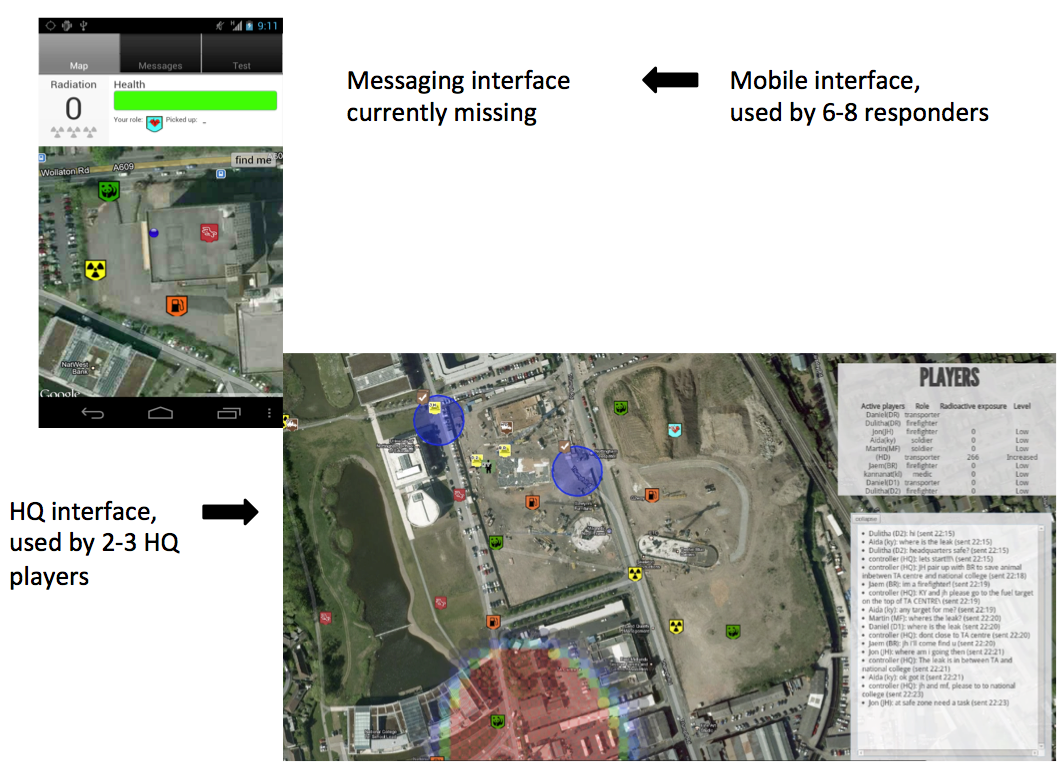
\includegraphics[width=1\textwidth]{img/conclusion/study1interface}
  \caption{Interface of study 1}
  \label{fig:study1interface}
\end{figure}


The 1st study discovered several flaws of the initial interface, which leads to a number of design requirements. 

\begin{enumerate}
	 \item The interface should support quick acknowledgement and feedback in communication channel.
	 \item The interface should freshness of messages in communication channel.
	 \item The interface should provide support for geo-reference.
\end{enumerate}

A set of changes in the 2ed version (used in study 2) of AtomicOrchid are partly inspired by the requirements (see figure \ref{fig:study2interface}). In 2rd version, all targets are identified by unique task ids to support geo-referencing. Text messages in broadcasting channel are labelled by time stamp to flag potentially outdated information. With introduction of planning agent, the interface also supports quick feedback to the agent with one button press. To integrate agent planning support, a new tab (``task'') in implemented in the mobile app to show a text-based description of agent task-assignment. In HQ interface, the agent assignments can be revealed on request of the HQ players (HQ clicking on "show task" button).\\

\begin{figure}[H]
  \centering
  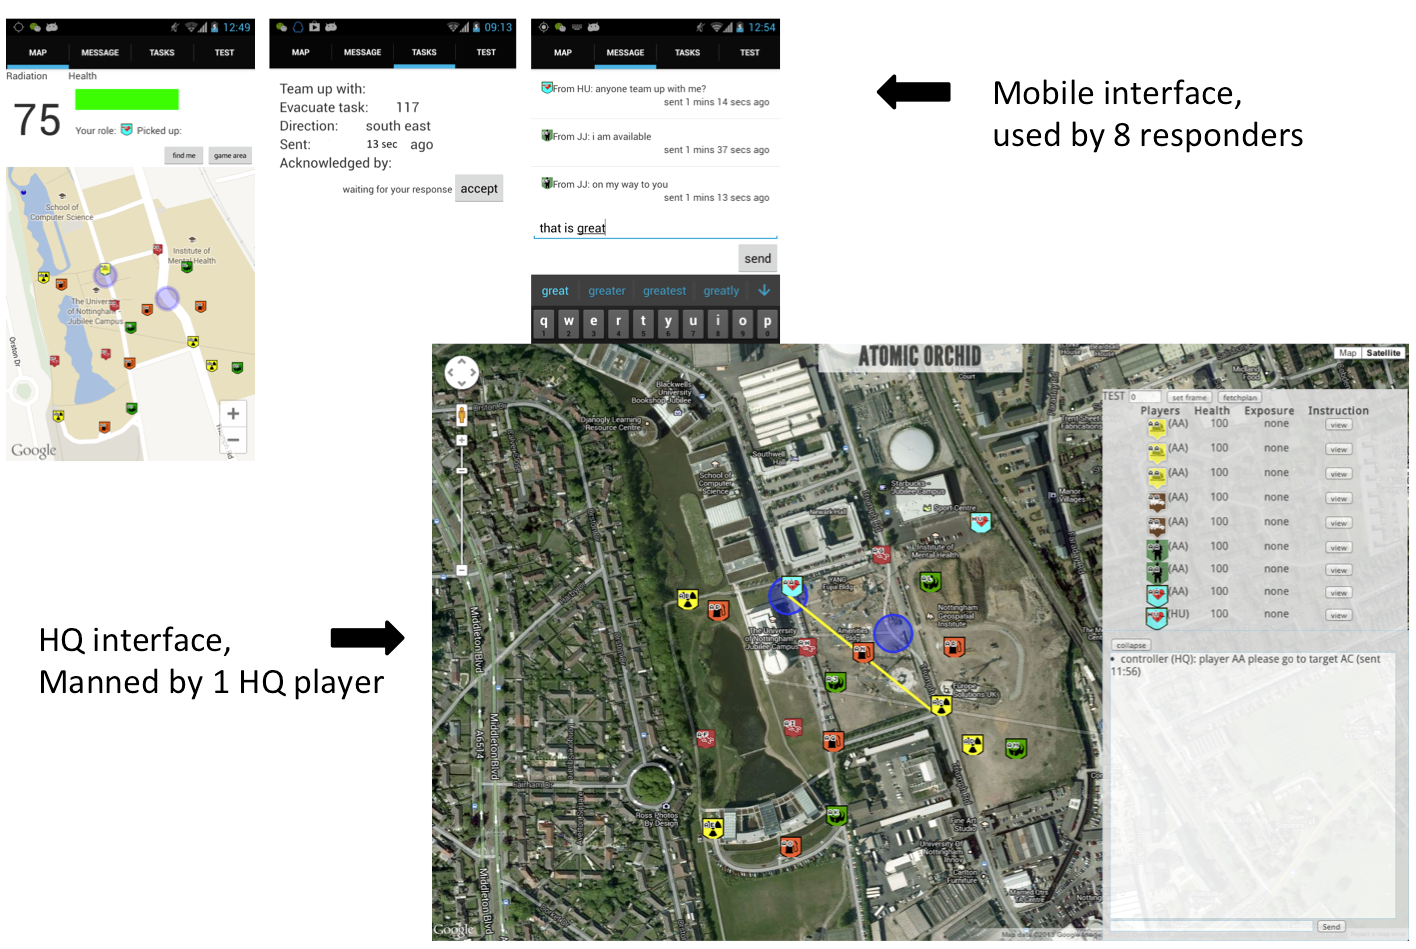
\includegraphics[width=1\textwidth]{img/conclusion/study2interface}
  \caption{Interface of study 2}
  \label{fig:study2interface}
\end{figure}

The result of the 2ed study revealed that interface level support for HQ intervention is missing in the 2ed version of AtomicOrchid. It is believed that the requirement for interface intervention support would also be important in the In-the-loop (the 3rd) study). Therefore, a task assignment (see figure \ref{fig:study3interfacemobile}) interface are introduced to enhance the HQ's ability to intervene the task planning. A task-specific communication channel is also introduced in the interface for players to avoid information overload in broadcasting channel. Compared to previous HQ interfaces, the operations on the task assignment interface is a lot more complicated. Therefore, one HQ player is dedicated to operate the interface and another player is provided with 2ed version of HQ interface by providing situational awareness and handling broadcasting messages. 

\begin{figure}[H]
  \centering
  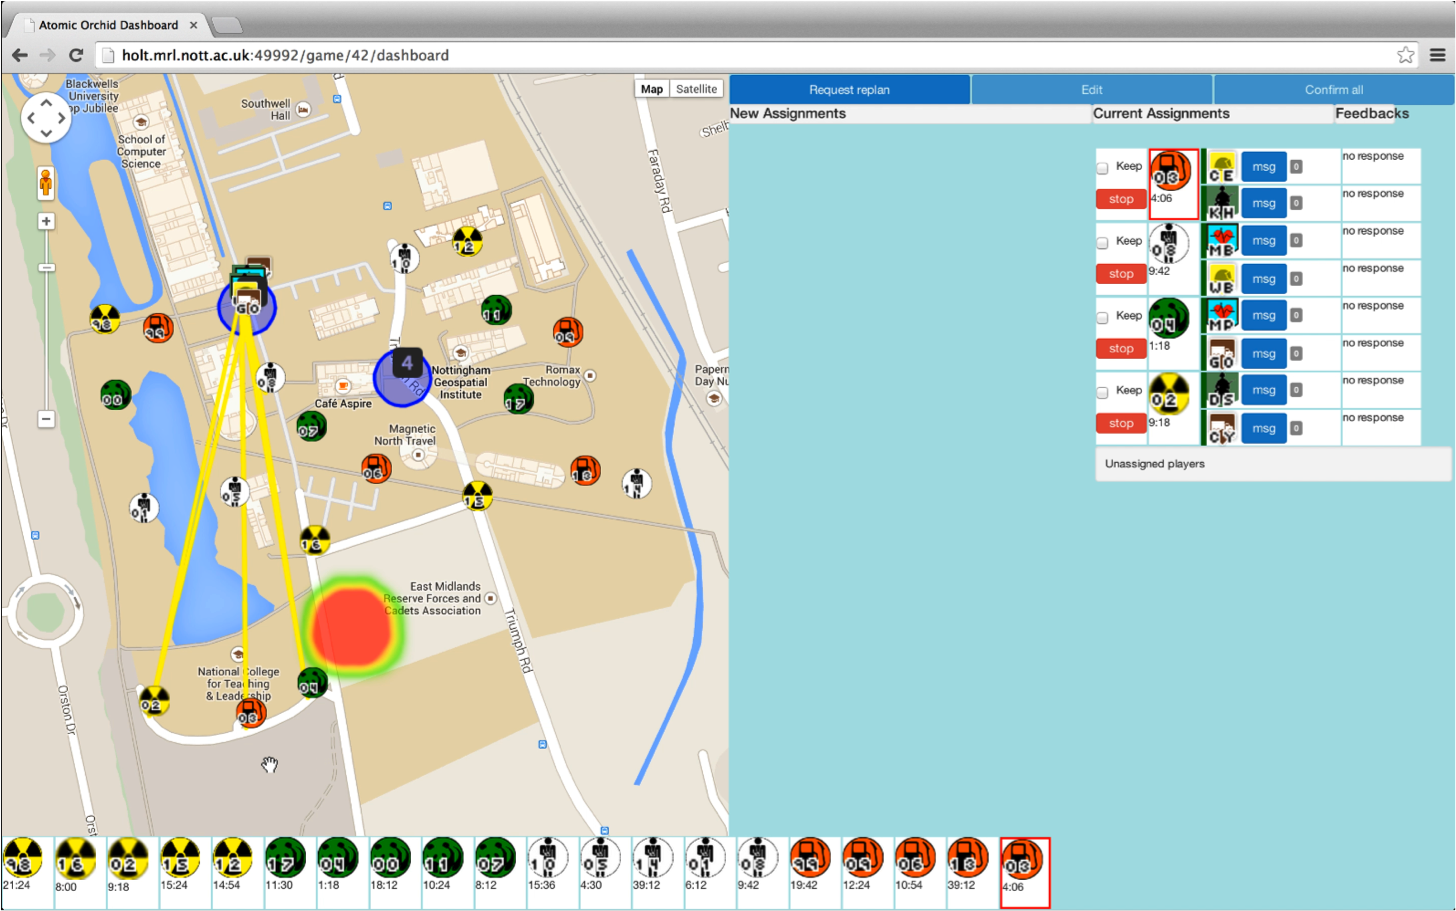
\includegraphics[width=1\textwidth]{img/conclusion/study3interfaceHQ}
  \caption{HQ Interface of study 3}
  \label{fig:study3interfacehq}
\end{figure}

For mobile interface, the tabs of ``staus'' and ``chat'' kept unchanged from the version 2 (named ``map'' and ``messages''). The task interface is enhanced by a map-based presentation of task assignment and the task-specific chat box is displayed below the assignment (see figure \ref{fig:study3interfacemobile}.

\begin{figure}[H]
  \centering
  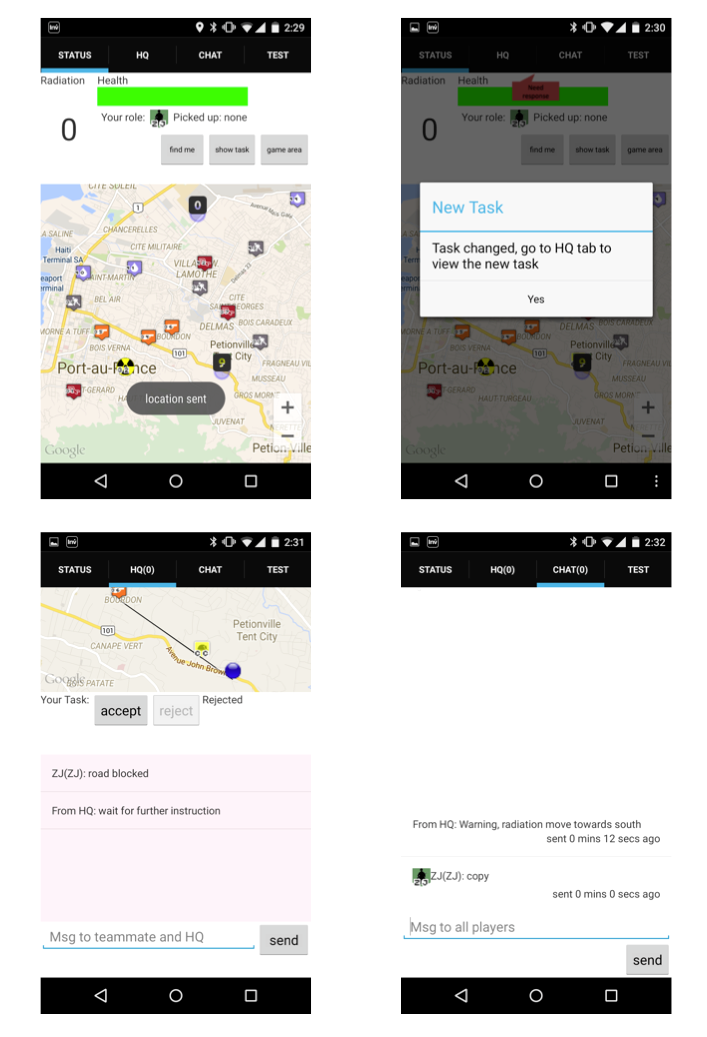
\includegraphics[width=1\textwidth]{img/conclusion/study3interfaceMobile}
  \caption{Mobile Interface of study 3}
  \label{fig:study3interfacemobile}
\end{figure}
\section{Summary of interactional issues}\label{sec:conclusionIssue}
There are a number of interactional issues emerged from the field observations of the three studies. This section will reflect on interactional issues related to 3 themes including Division of labour, common ground, and accountability.

\subsection{Division of labour}\label{sec:conclusionHH}
The On-the-loop and In-the-loop interaction designs have been trialled in two studies. The section will reflect on some of the findings related to the two interaction design patterns. \\

To recap, the main distinction between the two interaction design is the extent to which the human HQ is involved in routine task planning. The On-the-loop  argues the minimal involvement of human HQ, leaving the agent to deal with the planning. HQ only need to deal with occasional contingencies. The In-the-loop requires constant HQ agent interaction to ensure the planning quality. Guided by these two patterns, detailed system design has been implemented.\\

\begin{figure}[h]
  \centering
  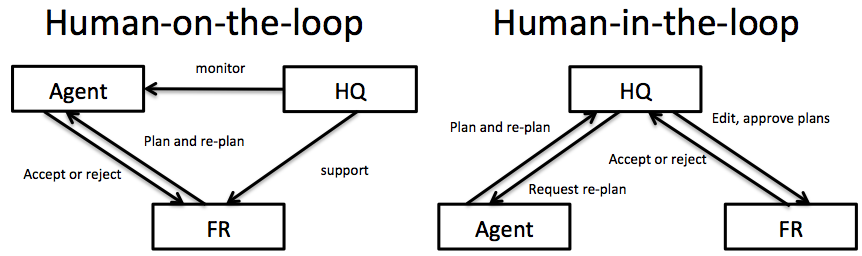
\includegraphics[width=1\textwidth]{img/conclusion/huilvshuol}
  \caption{On-the-loop vs In-the-loop}
  \label{fig:huilvshuol}
\end{figure}


There are several performance differences between the In-the-loop and On-the-loop studies. Direct comparison of performance between In-the-loop and On-the-loop is not applicable because the study 2 introduces a number of interface support (see figure \ref{fig:huilvshuol}) that influences team performance as well. However, the difference of performance can still leads to some implications of interaction design.\\

\begin{enumerate}
\item In-the-loop design as an option to reduce unnecessary task interruptions \\
As we have summarised in section \ref{sec:huilimperfection}, there are evidence showing that the HuOL design is more likely to cause extra coordination overhead when compared to the In-the-loop design. In study 2, HQ has been observed to deliberately avoid unnecessary task interruptions and team reformations caused by agent planning. It can be argued that the difference is simply caused by lack of reliability of the agent. Advanced agent planner which can better model the social process involved in task changes and take into account the possible overhead. However, given the social process might be hard to be modelled, the In-the-loop design can be useful to overcome the agent's limitation and utilise its capability at the same time.  

This option doesn't comes with no cost. On one hand, it increases workload of HQ player because need to check each instruction proposed by agent. HQs sometimes failed to recognise task interruptions even with interface highlighting support, which suggest HQ can not help to eliminate all the unnecessary interruptions. Effectiveness of HQ may also depend on a balanced workload. In a multi-tasking control room environment, it is critical to balance the the workload HQ. Therefore, we need to carefully consider the trade-off between the increase of workload and the reduction of task-interruption \\


\item The In-the-loop design may help maintain higher situational awareness [Need expand in study chapter]\\
As HQ is responsible for review and approval in In-the-loop design, they are found to maintain higher situational awareness when compared to the On-the-loop design. The observation is consistent with a well observed phenomena that the Human operator controlling a highly automated system is likely to loss situational awareness. [So?] \\

\item HQ's ability to intervene agent planning is required for both In-the-loop and On-the-loop design pattern.\\
Compared to In-the-loop study, the HQ players in On-the-loop study are found to struggle to intervene the planning process. This performance difference can not be directly linked to the distinction between In-the-loop and On-the-loop. In On-the-loop study, the only way for HQ to intervene the planning is to send unstructured text messages in broadcast channel. HQ's ability to intervene has been greatly enhanced by a set of interface support introduced in the In-the-loop study. Some of the interface support is inspired by the implications from On-the-loop study. It highlights the need of interface support for HQ intervention because both In-the-loop and On-the-loop requires HQ get involved when necessary. \\

\item Greater human involvement may introduce human mistakes. \\
Compared to On-the-loop, the In-the-loop design is more likely to introduce human mistakes as the design advocates greater human involvements. There is a case of  human "death" occurred  when field players were trying to follow a human generated plan in the In-the-loop trial.  Although there are lots of factors contributing to the `death' case (e.g. insufficient training for field play, communication breakdown), the task assignment is thought to be too risky and not recommended by the agent at the first place. It is believed that the chance of human mistakes can be reduced by appropriate design interaction which help establishing the `common ground' between human and agent. However, such a design would not be as easy task as it involves multiple design trade-offs  (see section \ref{sec:conclusionCG})[Need to expand in study section]

\item Model of Accountability

\end{enumerate}

To sum up, the reliability of agent could be one factor when considering interaction design[]. The improvement of reliability can reduce required human involvement, thus, allowing the HuOL design. However, in this PhD study, we assume human behaviour and disaster environment can be hard to be perfectly modelled. Therefore, In-the-loop design can be employed to overcome the (limited) reliability of the agent. Secondly, situational awareness of HQ can be important for both In-the-loop and On-the-loop design, though the study shows In-the-loop design help HQ to maintain situational awareness. Further, the interface support for HQ intervention has been proved to important in both In-the-loop and On-the-loop settings. Finally , a greater human involvement in planning (In-the-loop) are likely to introduce more human mistakes. The issue highlights the need for effective information sharing between human and agent, which help establishing the `common ground' for coordination. \\


\subsection{Establishing Common Ground} \label{sec:conclusionCG}
Establishing a common ground between human and agent has emerged as a common topic in discussions of both study 2 and study 3. The section will summaries the implications on establishing "Common Ground" from the two agent studies. \\

The "common ground" could be improved from 2 aspects:  1) Appropriate interaction design which allow human operators to understand the agent. 2) technical advancement in terms of algorithm and modelling techniques which enable agents to model human behaviours and process human feedbacks (e.g. agent being able to consider social cost of team reformation). The latter concerns about technical aspect of agent design which is beyond the scope of this PhD work. Therefore, this section will focus on building "Common ground" from the the perspective of interaction design. \\

In both study 2 and 3, the agent behaves like a "black box" which gives the results (task allocation). The interface only exposes the results of agent for HQ to monitoring. Through our observations in chapter \ref{ch:studytwo}, \ref{ch:studythree}, we find there could be some extra information shared between human and agent to improve planning.\\

The HQ players is found (section x.x.x) to occasionally make some forward planning for field players. Because the forward planning is also performed by the agent to derive current plan, the information could be shared so that the HQ players can be provided with the agent suggestion when doing forward planning.\\

The reasoning behind current task allocation would also be useful for sharing. In chapter \ref{ch:studythree} , HQ is found overriding agent plans, which leads to undesirable results. The HQ is also found being confused when agent stop assigning tasks to players with low health. Exposing internal reasoning of the agent can help the HQ to make informed decisions. \\

Misunderstanding between agent and human is also observed in the feedback loop in study \ref{ch:studytwo}. Firstly, human respond do not know how agent is going to handle the rejection. The try to use rejection to reverse back to previous tasks, while the agent will give them more new instructions. Secondly, it is unknown to field responders that their rejection will cause replanning for the whole team which can lead to lots of costly task interruptions. Therefore, information indicating consequence of interface interactions should be also made available to human to facilitate accountability and ensure informed decisions. \\

Although, we have identified a range of information which is missing for establishing "Common Ground", presenting the information could be also challenging. The information should be delivered in right form (e.g text, visualisation, dialogs) and in right time (e.g. pop up or on HQ request?)[] Especially in the multi-tasking, time-critical settings like AtomicOrchid, multiple sources of information can compete for attention of the human operator. Information overload could be a real danger of interaction design in this setting. Therefore, the  way for exposing agent's information and its human performance consequence may need to be further studied.   \\


\subsection{Faciliating Accountability}\label{sec:conclusionAC}

\section{Limitation}
This section will outline some of the limitations of this PhD work. \\

By following a serious mixed reality game approach, the game AtomicOrchid is used to simulate some key factors of the distributed, time-critical task setting.  The fictitious game scenario can not completely mirror the setting of disaster operations. Firstly, the time-scale of planing is match longer in a rescue and reconnaissance mission (from hours up to days), while the AtomicOrchid only have 30 mins time-scale. Secondly, the disaster response teams always priorities critical tasks according to code of conduct (e.g. task with human injuries will always be prioritised. see section of RG interview). Therefore, the game objective of maximising targets saved may not match real goal of DR team.  \\

Further, the seriousness of the simulation can also be a limitation of game approach. Participants are frequently observed to laugh and make jokes about their health values (life), which indicates they take the trials as a recreational experience. Therefore, the participants maybe less concerned about risk and life threats, when compared to real disaster setting. \\

The untrained participants are recruited for the field trials. We anticipate that the behaviours of players in the game may change with their training experience. Further, the professional responders can also behave differently because they have high level of training, real experience of DR operations, different code of conduct and organisation structure.\\


Overall, the PhD work employed a game approach, which has a number limitations in terms of game scenario, participants' altitude, and participants' selection.  We can not claim the observations of human behaviours would be exactly the same as what happens in the real disasters. However, we argue that the game-based approach managed to introduce some critical factors of DR operations, including time pressure, distributed team setting, and the mental/physical stress. Compared to computational simulation, the field trials can reveal rich human-system interactions under time and spatially constrained task environment. Therefore, we argue the observations from game trials are still valid and can be used to generate design implications for future HACs systems. 

\section{future work}
Following the limitations and contributions of the thesis, its impact can be extended into future work in several possible ways.\\

Firstly, the planning agent itself can be improved with various AI technologies. For example, the agent in this study does not consider the social cost of re-teaming and task interruption. Some user modelling technologies such as [] have potential to be used predict human behaviour, which in turn, helps to model the social cost of re-teaming and task interruption  [] . However, when agent is enhanced by new AI technologies, it is unknown whether the new capabilities would hinder or improve team coordination and how the interaction design should be adapted to support the new capabilities.  Therefore, one future direction of this PhD study is to incrementally enhance agent capabilities and conduct observational studies to gain insight into the implications of the new enhancement on the interaction design.\\

The game can be re-engineered so that the game setting can be better grounded in the real practices of disaster operation team. In order to do that, the close collaboration with disaster response teams may be required. The collaboration with Global Rescue happened  in the late stage of this this PhD work, which help us to identify some potential improvement of the game setting. Firstly, the targets are not always equally important. For example, humna injury will typically be prioritised. Considering different weighting on targets can make the game setting more realistic. Secondly, radio rather then text messages is the communication modality used by operation teams, which may have impact on our behaviour observations. Thirdly, the AtomicOrchid assume constant connectivity between HQ and field responders, but the disaster operations are often characterised by intermittent communication. Therefore, it would also be useful to simulate the intermittent communication in AtomicOrchid.  \\

In a similar vein, the subjects of study can be changed to professional responders in order to better elucidate human behaviour in real disaster operation.  As we believe that the trained professional responders may behave differently with the general public. It would be desirable to recruit professionals in the future work to validate the findings of this PhD study.\\

In terms of the methodology, more field trials can be conducted in order to carry out statistically robust quantitative analysis. If there are more field trials, quantitative analysis can compliment the qualitative interaction analysis in some aspects. For example, the statistical difference in terms of games results (including players death, targets saved) can be used to imply effectiveness of interaction designs. Also the social cost and workload of HQ may also be quantified (?) to give insight into the impact of interaction designs on the team performance. (more?)\\

The studies have highlighted the trade-off between establishing common ground and information overload (see section x). I believe further studies may be needed to unpack  how the trade-off affects team coordination and develop systematic approach for system designer to balance trade-off. \\  

Moreover, the interaction designs are not limited to the On-the-loop and In-the-loop. Contribution of this PhD work can be extended by exploring some middle-ground designs. For example, the agent can be given the responsibility to decide when to perform a re-plan (as it is in the On-the-loop design), but also send the instructions to HQ for approval (as it is in the In-the-loop design).\\

It should also be noted that the centralised planning support is only one kind of agent planning support technology among many. For example, the planning support can also be decentralised. The planning agents can be built into personal assistant devices for every field responders. The change of agent technologies certainly have implications on interaction design. New interaction design pattern can be devised and adopted with the change of agent technologies. Therefore, this PhD work can potentially be extended with exploration of different agent technologies.\\ 

Further, this work contributes to the research paradigm of HACs system (see section x) by studying the interaction between one centralized planning agent and a disaster response team. However, the HACs researchers envision a scenario in which large amount of computational entities (including both software agents and embodied agents such as rescue robots ) and human teams collaborate at large scale. For future work, there is a potential to extend AtomicOrchid incorporate multiple agents and human teams to study multi-agents and human interaction.\\




